\section{Background and methodology}
We begin by providing an introduction the Vine platform, then describe the datasets of micro videos we crawl from Vine and finally give details of the features we extract from the micro videos.
\subsection{Introduction to Vine}

Vine\footnote{http://vine.co} is a video sharing platform owned by Twitter, where users can create and share videos (called ``vines'') up to 6 seconds long, a constraint which was designed with the goal of inspiring ``creativity''\footnote{http://blog.vine.co/post/55514427556/introducing-vine}. Vine is primarily used as a mobile app, although a Web interface as well as an Xbox Live interface is available to view the videos. Users may create vines and upload them to the platform (typically through the Vine mobile app), view vines created by others, and follow other users whose vines they find interesting. 

Users see vines created by others in one of several tabs: The home tab shows a personalised and social feed of videos created by those that they follow. The explore tab shows 20 feeds and channels. Eighteen of the channels are category-specific, such as `Comedy', `Music', `Animals', `Weird', `Sports', `Arts' etc\., and appeal to different kinds of users based on their specific interests. Vines are  assigned to specific channels by their creators. The remaining two channels are termed by Vine as 'popular-now' and 'on-the-rise',  and are curated channels containing videos that have proven to be of of wider appeal to the entire Vine population. 

As with other modern content-sharing platforms, there is a social aspect: viewers can follow others whose vines they find interesting, `like' or share interesting vines by `revining' (i.e., reposting) the vines, and commenting on them. The numbers of likes, revines and comments are a measure of the popularity of a video. Uniquely, Vine plays videos in a loop, going back to the beginning after reaching the end. Loops are repeated as long as the focus is on that video (e.g., video is active on the mobile phone screen if using the Vine app, or mouse is on the video in the web version). Thus, letting a video play for more than one loop can be a sign of engagement. Therefore the platform also tracks and reports in real time the aggregate number loops across all users. 

%some may be featured on playlists on the Vine home page;feed generated for logged in users, which shows Come up with a description of what a reader needs to understand about vines to understand our paper - in particular mention and define reposts/revines, how we use them interchangeably; loops and likes.

%How a Vine surfaces to followers: through the home feed, you can see videos of those whom you follow. If it is tagged, and tag becoms as a trend, then it shows up in the trending page. There are 18 channels or categories. If you assign to a channel, then it shows up in the global list of channels/categories. 



\subsection{Dataset description}\label{sec:dataset}
\begin{table}[hbt]
\centering
  \begin{tabular}{l|cccc}
    \thead{Dataset} & \thead{\shortstack{Vines\\ (total)}} & \thead{\shortstack{Loops\\ (median)}} & \thead{\shortstack{Reposts\\ (median)}} & \thead{\shortstack{Likes\\ (median)}} \\
    \hline
    POP12K & 11448 & 318566  & 2173 & 7544  \\
    ALL120K & 122327 & 80 & 0 & 2 \\
    INSTA15k & 14568 &  2089  & N/A  &  489\\
  \end{tabular}
  \caption{Summary characteristics of datasets used}
  \label{tbl:dataset}
\end{table}


The data used in this paper is summarised in Table~\ref{tbl:dataset}, and was collected in two phases as described below: 

\paragraph{Popular videos dataset} First, we collected $\approx$ 12,000  videos which have been marked by Vine as `popular', by tracking the `popular-now' channel\footnote{https://vine.co/popular-now} over a three week period in Dec 2015, and downloading all videos and associated metadata once every six hours, and removing any overlapping videos from the previous visit. The crawling period was chosen to ensure that consecutive crawls have an overlap of several videos, and this sufficed for all visits made to the website during the data collection period; thus the dataset we collected is a complete collection of all `popular-now' vines during the 21 days under consideration. %After removing all duplicates, a total of \textbf{XXX} popular videos were collected. 

Vine does not disclose the algorithm used to mark a Vine as popular; yet we observe (see Table~\ref{tbl:dataset}) orders of magnitude more loops, reposts and likes in the popular-now dataset than in the non-popular dataset. Thus we believe that the algorithm used by Vine to select vines for the 'popular-now' channel is strongly affected by the numbers of loops/revines/likes. Note that the numbers of loops etc. were collected at the time of crawl, within a maximum of six hours of being posted on the 'popular-now' channel, which limits the possibility that the counts increased \emph{as a result} of being featured on the popular-now channel. In the rest of the paper, we use the counts in the popular-now dataset to calibrate the definition of `popular'. While there is a possibility that this is a biased proxy for global popularity, it nevertheless provides a baseline against which to compare all videos.

\paragraph{All channel videos dataset} In the second phase, we collected 
videos accessible from each of the 18 global Vine channels or categories%\footnote{https://vine.co/api/timelines/channels/<channelNumber>/recent?size=100} 
 over a period of {8 weeks} from {Aug 16 to Oct 12  2016}. Again, a crawling period of six hours was chosen for consecutive visits to the same channel, and the 100 most recent vines were fetched with each visit. As shown in Fig.~\ref{fig:download-fraction}, the  vines returned has a significant overlap with vines fetched from the previous visit. Thus we believe that our dataset captures nearly all videos uploaded to Vine and assigned to a channel. The only exception is the extremely popular comedy channel, for which we nearly always find more than 100 new videos (we only download the 100 most recent videos for the comedy channel). In total, this results in a dataset of $\approx$120,000 videos. We track  loop, reVine and like counts  over time, periodically updating each video's counts every three days until the end of  data collection.
  
Note that while we obtain nearly all videos across the channels, our dataset does \emph{not} capture  \emph{all} videos uploaded to Vine -- Vine creators do not need to assign a video to a channel. However, due to the Vine platform structure,  vines that are not in channels have near-zero probability to get seen by other users. % and we do not discover any vines not in channels. 
We use channels to restrict ourselves to vines which have a chance to get exposed to a reasonably global audience of those interested in a topic category, and therefore to vines that have a higher potential for garnering high like/revine/loop counts. 

\paragraph{Instagram Video dataset} Finally to more than one source for understanding the new paradigm of micro videos, we collect Instagram videos by designing a crawler that tries to search instgram users by seeding the search query with user names found on Vine. We end up crawling pages of 4500 users out of  which 150 are verified Instagram users which mean these users are public figures and are validated by Instagram themselves.  To track user engagement, we track all videos to see their cumulative activity after 3 weeks since upload. This is to have uniformity in comparison of engagement between Vine and Instagram posts. 

\begin{figure}[htb]
	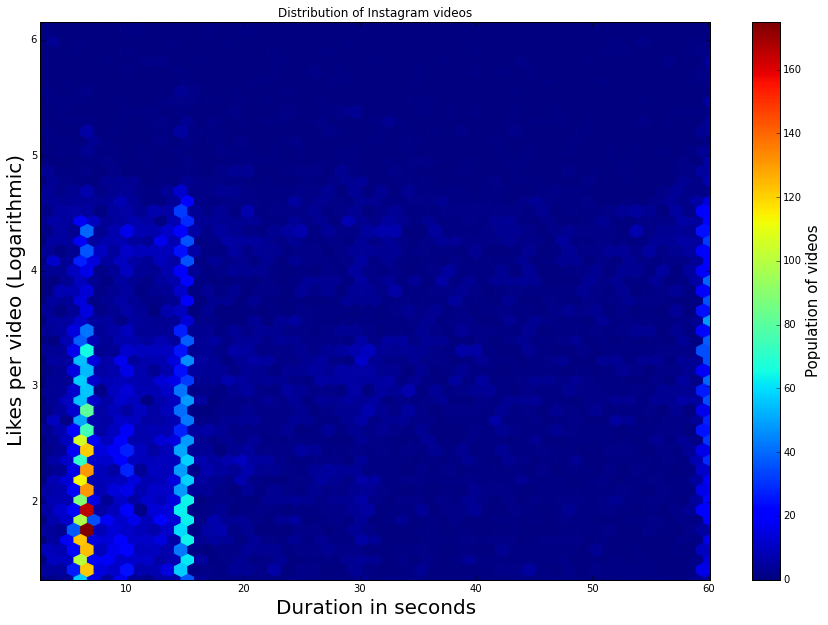
\includegraphics[width=0.9\columnwidth]{plots/InstaEngagementHeatmap}
	\caption{A 2 dimensional distribution heat-map of the 15k videos crawled from instagram. The plot clearly shows a trend, where despite having a relaxed time constraint for videos (1 minute) users and consumers are converging on shorter formats of duration lengths between 5 and 20 seconds. }
	\label{fig:download-fraction}
\end{figure}

  %
%\begin{figure}[htb]
%  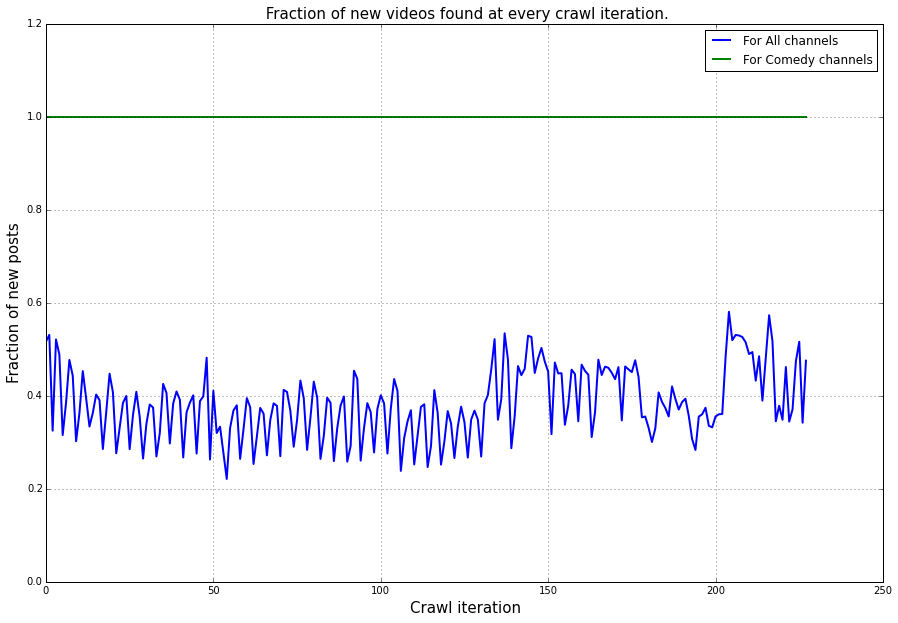
\includegraphics[width=0.9\columnwidth]{plots/UniquePostDownload}
%  \caption{Fraction of new videos since last visit amongst the videos whose metadata was fetched by requesting for the 100 most recent videos from each channel is consistently less than 1, suggesting that the dataset contains nearly all videos from most channels. The only exception is the comedy channel, which consistently has more than 100 new videos (fraction of new videos is nearly always 1).}
%  \label{fig:download-fraction}
%\end{figure}



%
% 
%Because we expected the popularity distribution of videos to follow a heavy-tailed distribution, the number of popular vines 
%we wanted substantial samples qualified to be popular by Vine standards. Hence we crawled the Vine popular channel over 3 weeks to collect 12000 unique popular videos. These videos would make our gold standard dataset (POP12k). Further We collected an additional 120,000 videos which were at a very early stage of their lifetime over 8 weeks (UNPOP120K) . These videos were not classified to be popular becasue of their nascent nature. We tracked these videos over 4 weeks for their popularity metrics and user metrics.
%Along with the videos we collected metadata about the video, the profile of the user, and the metadata of the user who posted the video. 

%The popularity distribution of the whole dataset follows as expected a zipf distribution. The Fig. 1 shows the distribution of likes and repost counts of the collected videos on al og scale. Videos with 0 likes or reposts were given a marginal 1 like to avoid undefined logarithms. 
%
%\begin{figure}[!htb]
%\centering
%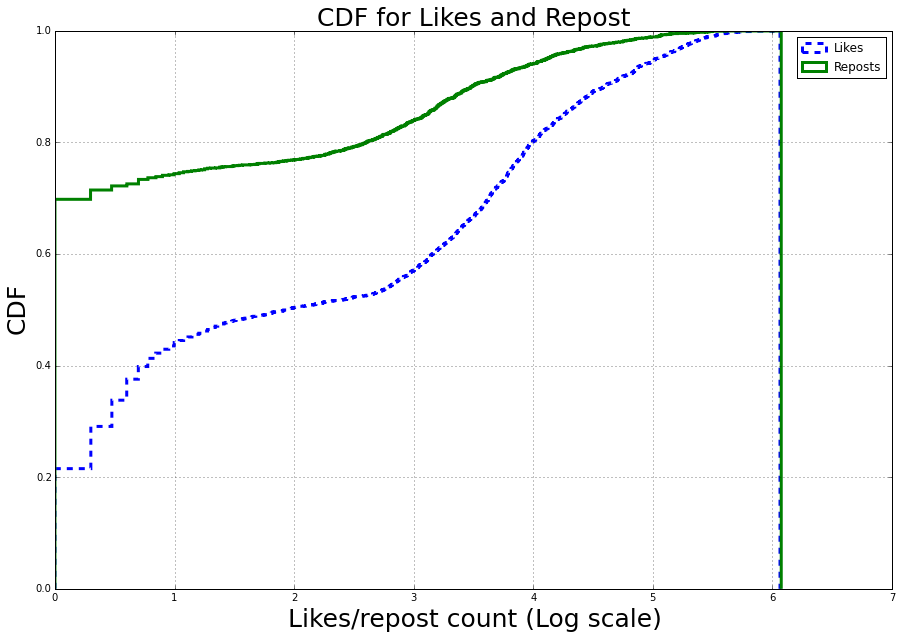
\includegraphics[width=\columnwidth]{plots/CDF_Like_reposts}
%\caption{\textsl{ CDF of Like count and Repost count.} \textbf{The values are normalized and on a Logarithmic scale. As expected from a long tail distribution of metrics like popularity, the dataset has a lot of videos with zero likes and reposts. Such videos are synthetically given one like and repost to avoid undefined values}}
%\label{fig:CDF_posts}
%\end{figure}

%\paragraph{Third party datasets}
%We also used several third party datasets, to do a comparative study of Vine with other kinds of social media: For comparison with  image-based social media, we use the popular MIR-Flickr dataset \cite{huiskes08} which is an open source dataset of over 25,000 Flickr images,  which are known to be popular (i.e., with high  ``interestingness''\footnote{https://www.flickr.com/explore/interesting} rating). %, and are verified to be aesthetically pleasing. This was achieved by making sure that they were ranked high . These images were used as a baseline for static web images in the comparison study.
%To compare with video-based social media, we used a dataset of  $\approx$400 viral youtube videos \cite{Jiang:2014:VVS:2578726.2578754}. For our work with frame sentiments, we use a  dataset provided by the Sentibank researchers \cite{jou2015visual,SentiBank} for baselining the performance of our detector for detecting frame sentiments in micro videos.


